\chapter{Hardware design}
\begin{large}
TODO::Beskrivelse af hardware design overordnet
\end{large}

\section{Encoder}
Encoderen, også omtalt som senderenhed, er den del af systemet der genererer X10 kommandoen og sender den ud på det eksisterende el-net. Et højpasfilter der lader 120 kHz burst passere mens det blokerer for nettets 50 Hz signal, udgør sammen med en zero crossing detector hele hardwaren for encoderen.

\begin{large}
TODO:: billede af burst ud på nettet!!
\end{large} 

\newpage

\subsection{Højpasfilter}

\begin{figure}[htb]
  \begin{minipage}{0.45\textwidth}
    \centering
      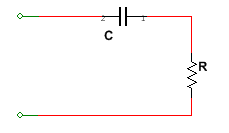
\includegraphics[width=\textwidth]{billeder/HWdesign/HP_UV}
      \caption{Højpasfilter uden værdier}
    \label{fig:HP_UV}
  \end{minipage}
  \hspace{0.1\textwidth}
  \begin{minipage}{0.45\textwidth}
    \centering
      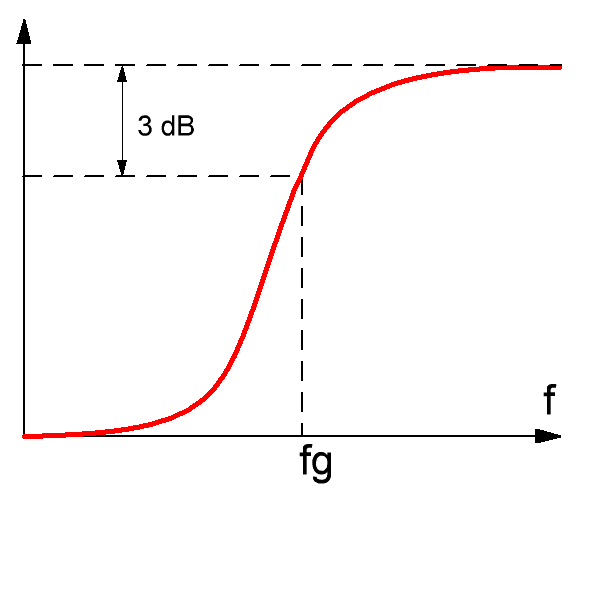
\includegraphics[width=\textwidth]{billeder/HWdesign/HP_KURVE}
      \caption{Kurvekarakteristik for højpas filter}
    \label{fig:HP_KURVE}
  \end{minipage}
\end{figure}

For at sende X10 kommandoer ud på det eksisterende 50 Hz el-net er det nødvendigt at koble elektroniken direkte herpå og eftersom det elektronik ikke tåler de høje spændinger fra nettet, er det nødvendigt at blokere det signal, men stadig at kunne sende de 120 kHz ud. Dette løses med et højpasfilter.

Den ønskede knækfrekvens skal ligge omkring de 120 kHz for at opnå mindst dæmpning herpå. Ved denne knækfrekvens skulle 50 Hz signalet være ubetydelig lille efter filteret. 

Kondensatoren forudbestemmes for beregningerne til en værdi på 0,1 nF.

\begin{align}
R_1 = \frac{1}{2 \cdot \pi \cdot f_c \cdot C } = \frac{1}{2 \cdot \pi \cdot 120000 \cdot 0,1 \cdot 10^{-6}} = 13,26 \Omega
\rightarrow R_1 > 13,26 \Omega
\end{align}
$R_1$ vælges da til 14 $\Omega$

Med den beregnede modstands værdi er det endelige schematic færdigt som det ses på figur \ref{fig:HP_MV}

\begin{figure}[htbp]
	\centering
	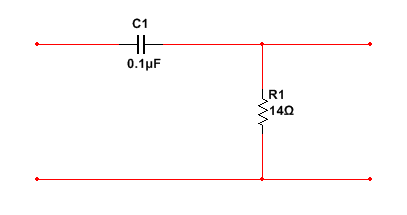
\includegraphics[width=0.50\textwidth]{billeder/HWdesign/HP_MV.png}
	\caption{Højpasfilter med værdier}
	\label{fig:HP_MV}
\end{figure}

\newpage
  
\subsection{Zero Crossing Detector}
\begin{figure}[htb]
  \begin{minipage}{0.45\textwidth}
    \centering
      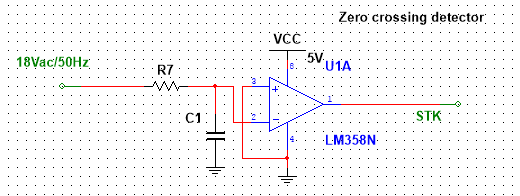
\includegraphics[width=\textwidth]{billeder/HWdesign/ZC_UV}
      \caption{Zero crossing detector uden værdier}
    \label{fig:ZC_UV}
  \end{minipage}
  \hspace{0.1\textwidth}
  \begin{minipage}{0.45\textwidth}
    \centering
      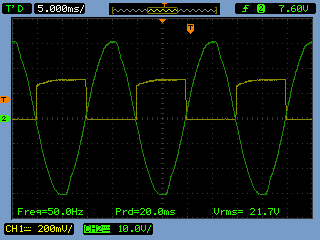
\includegraphics[width=\textwidth]{billeder/HWTest/Encoder/Encoder_zerocross}
      \caption{Scope billede af Zero crossing detector, CH1(indgangssignal), CH2(Udgangssignal)}
    \label{fig:Encoder_Zerocross}
  \end{minipage}
\end{figure}

Zero crossing detectoren har til opgave at detektere nulgennemgang, det er et krav for at X10 protokollen kan virke. Der er placeret en Zero crossing detector både på Encoderen og Decoderen, da begge disse består af et STK-kit der kræver information om nulgennemgang. Opbygning kan ses på overstående figur \ref{fig:ZC_UV}, vi har anvendt en operationsforstærker af type LM358N, som toggler udgangssignalet ved hver nulgennemgang se figur \ref{fig:Encoder_Zerocross}. Operationsforstærkerens positive ben er koblet til stel for at lave et triggerniveau til 0 V.

Modstanden $R_7$ sidder der bl.a. for at beskytte Zero crossing detectoren mod 18 VAC nettet, men sammen med kondensatoren udgør den også et lavpasfilter. Under implementeringen opdagede vi at der kom støj ind på Zero crossing detectoren, og dette problem løste lavpasfilteret. 

Da vi ønsker at dæmpe 120 kHz signalet, designes lavpasfilteret ud fra en knækfrekvens på 1,0 kHz. 

\begin{align}
R = \frac{1}{2 \cdot \pi \cdot f_c \cdot C } 
\end{align}

Der vælges en kondensator med en værdi på 150 nF. Med denne værdig kan modstanden i lavpasfilteret beregnes. 

Lavpasfilterets modstand:
\begin{align}
R_7 = \frac{1}{2 \cdot \pi \cdot \ 1000 \cdot 150 \cdot 10^{-9}} = 1061 \Omega
\end{align}
$R_7$ vælges da til 1,0 k$\Omega$

Med alle de beregnede komponentværdier kan det endelige schematic designes. Det endelige design er vist på figur \ref{fig:ZC_MV} 

\begin{figure}[htbp]
	\centering
	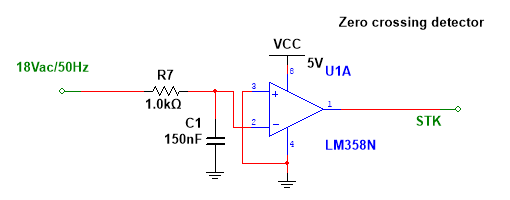
\includegraphics[width=0.70\textwidth]{billeder/HWdesign/ZC_MV}
	\caption{Zero crossing med værdier}
	\label{fig:ZC_MV}
\end{figure}

\newpage

\section{Decoder}
Decoderen som er den del i systemet der omdanner burst fra encoderen til X10 kommando er bygget op af et båndpasfilter, zero crossing detector og en envelope detector. I starten af kredsløbet sidder båndpasfilteret. Dette blokerer for 50 Hz nettet og forstærker 120 kHz signalet der kommer fra encoderen. Herefter ledes signalet gennem envelope detector som omdanner burstet til et TTL signal.

\begin{large}
TODO: Billede af burst ind og TTL signal efter envelope..
\end{large}

\newpage

\subsection{Båndpasfilter}
\begin{figure}[htbp]
	\centering
	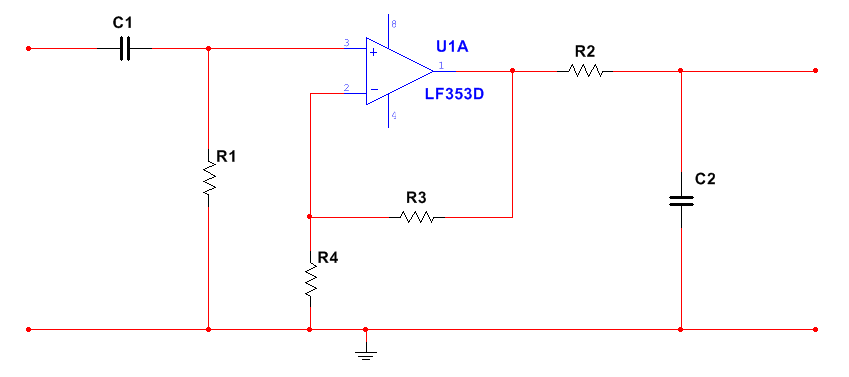
\includegraphics[width=0.70\textwidth]{billeder/HWdesign/BAANDPAS_UV.png}
	\caption{Båndpas uden værdier}
	\label{fig:BAANDPAS_UV}
\end{figure}

Båndpasfilteret har til opgave at filtrere alle signaler med frekvenser over og under 120 kHZ fra samtidig med at det forstærker signalet i båndpasset. Forstærkningen opnås ved at koble en ikke inverterende OpAmp med modstande, hvis størrelse afhænger af den ønskede forstærkning, mellem et højpasfilter og lavpasfilter som illustreret på figur \ref{fig:BAANDPAS_UV}.

Da vi ønsker at forstærke 120 kHz signalet, designes højpasfilteret således at knækfrekvensen udregnes til 110 kHz, og for lavpasfilteret beregnes en knækfrekvens på 130 kHz. 

\begin{align}
R = \frac{1}{2 \cdot \pi \cdot f_c \cdot C } 
\end{align}

Fælles for begge filtre vælges en kondensator med en værdi på 1,0 nF. Med denne værdig kan de to modstande i henholdsvis lavpas- og højpasfilteret beregnes.

Højpasfilterets modstand:
\begin{align}
R_1 = \frac{1}{2 \cdot \pi \cdot 110000 \cdot 1,0 \cdot 10^{-9}} = 1447 \Omega
\rightarrow R_1 > 1447 \Omega
\end{align}
$R_1$ vælges da til 1,6 k$\Omega$


Lavpasfilterets modstand:
\begin{align}
R_2 = \frac{1}{2 \cdot \pi \cdot \ 130000 \cdot 1,0 \cdot 10^{-9}} = 1225 \Omega
\rightarrow R_2 < 1224 \Omega
\end{align}
$R_2$ vælges da til 1,1 k$\Omega$

Da det ikke kan undgås at 120 kHz signalet bliver dæmpet både gennem højpasfilteret og lavpasfilteret er det nødvendigt at forstærke signalet ved hjælp af en LF353 OpAmp.
Ligningen for udregning af udgangsspændingen er som følgende:
\begin{align}
V_{out} = (1 + \frac{R_3}{R_4}) \cdot V_{in}
\end{align} 

Ved at vælge $R_4$ til 10 k$\Omega$ kan forstærkningen nemt reguleres med $R_3$.
Ved målinger på indgangssignalet før operationsforstærkeren kan vi fastslå indgangsamplituden til at være 8,0 V. Da udgangssignalet ledes gennem en diode der fjerner de negative halvperioder vil amplituden blive halveret gennem denne. Samtidig er der dæmpning i lavpasfilteret og der vil derfor være brug for en mere end en fordobling i forstærkeren. 

\begin{align}
R_4 = (\beta - 1) \cdot R_3 = (3 - 1) \cdot 10000 = 20000 \Omega
\end{align} 
$R_4$ er valgt til 20000 $\Omega$ så signalet derved bliver forstærket 3 gange.

Der er som nævnt valgt en LF353 OpAmp. Denne er valgt ud fra at den har en bred båndbredte, en hurtig sætte tid og lav støj på indgangene. 

Med alle de beregnede komponentværdier kan det endelige schematic designes. Det endelige design er vist på figur \ref{fig:BAANDPAS_MV} 

\begin{figure}[htbp]
	\centering
	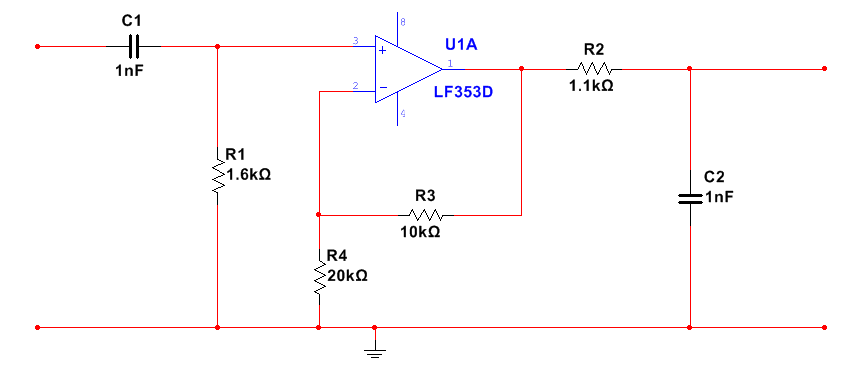
\includegraphics[width=0.70\textwidth]{billeder/HWdesign/BAANDPAS_MV.png}
	\caption{Båndpas med værdier}
	\label{fig:BAANDPAS_MV}
\end{figure}
 

\newpage

\subsection{Envelope Detector}
